\chapter{Flight Dynamics}
The primary responsibility of the Flight Dynamics team is to simulate the performance of both the launch vehicle and the payload, to inform other subteams of constraints that must be satisfied to achieve safe flight, and to make design decisions on all structures and control systems that directly influence the flight of the launch vehicle-payload system.

\section{Simulation Methods}
In order to ensure that predictions of flight performance, as well as insights into possible design improvements, are robust and well-informed, the team is using two different calculation methods to study the flight profile. The team is principally using OpenRocket for simulating the flight of the launch vehicle and predicting critical mission characteristics such as apogee, time to apogee, and total flight time, among many others. OpenRocket is a powerful, open-source rocket flight simulation tool. As it is the most robust and informative, cost-free flight simulation tool available, the team is using it as the primary consultant on aerodynamic design considerations and predicting if the launch vehicle satisfies mission requirements. In addition to predicting flight trajectories, from launch to landing, for various possible initial conditions, OpenRocket also provides baseline estimates for the launch vehicles's mechanical and aerodynamic properties, including pre- and post-burnout masses, drag and lift coefficients, CP and CG locations, stability coefficient, and many others. 
\\*
\newline
As another feature of its versatility, OpenRocket offers multiple customization options for running its trajectory simulations, such as various Earth models and time step size for the numerical integration. To confirm that the simulated trajectories are reliable, the team used two different Earth models, each with a different time step size. The simulation conditions the team used are summarized in the table below.
\FloatBarrier
\begin{table}[H]
\centering
 \caption{OpenRocket simulation conditions}
 \label{tab:FlightDynamics:SimulationConditions}
\begin{tabularx}{.5\linewidth}{llX}
\toprule
 \textbf{Condition} &  \textbf{Time step size [s]} \\
\midrule
   Spherical Approximation &    0.05 \\
    WGS84 &     0.01 \\
\bottomrule
\end{tabularx}
\end{table}
WGS84 (World Geodetic System 1984) is an ellipsoidal model of Earth, and is more accurate than the spherical approximation. Combined with a smaller step size, the trajectory simulation under the WGS84 model is expected to be more accurate than the simulation under the spherical Earth model.

\section{Flight Profile}
The flight profile for this mission features a relatively simple sequence of events.
Nominally at apogee of 4,450ft (and within 2 seconds after apogee), an ejection charge
in the tube coupler will separate the upper and lower body tubes and deploy the drogue parachute. This will be the only explosive separation event of
the entire flight. The main parachute will then deploy at 800ft (this is above the minimum
parachute deployment altitude of 500ft). This was determined to be the optimal altitude because it is high enough to reduce terminal velocity (and thus satisfy the landing kinetic energy requirement), while also being low enough to ensure an acceptable drift distance. 
\\*
\newline
Within two seconds of main parachute
deployment, the solenoid system in the fairing will trigger after the necessary RSO
permission is acquired. Since the nose cone is sized to fit loosely into the fairing, releasing the solenoids will allow the nose cone to slide freely from the fairing, from which point it will descend the remainder of the altitude independently. The nose cone will also be equipped with its own parachute, which will be secured with a Jolly Logic chute release. This device will be programmed to release the parachute at a pre-determined altitude, which is currently planned to be 400ft. Once the parachute is released, it will be unfurled by the low pressure region in the nose cone's wake. 
\\*
\newline
Immediately upon release of the nose cone by the solenoid system, the drone will passively slide out from the fairing under the influence of gravity, guided by a rail system to which it will be attached until deployment. Unlike the nose cone, the drone will be attached to the fairing by a lowering mechanism. This lowering mechanism will allow the drone to hang exposed to the free stream, enabling it to conduct the necessary observations to pass the on-board safety checklist, while using minimal thruster power. If the drone determines itself to satisfy the pre-specified conditions for safe flight, it will cut itself from the mechanism, and proceed with the mission.
\\*
\section{Simulation Results}
The flight profile was simulated in OpenRocket using a model of the rocket with numerous
design specifications (e.g. fin and body tube dimensions, material, and motor type), various initial
conditions, and even the exact coordinates of the launch site. Per competition requirements, the wind speed was varied between 0-mph, 5-mph, 10-mph, 15-mph, and 20-mph, and held constant during each simulation. To account for the launch rail being canted away from the crowd on launch day to offset wind conditions, the launch angle was also varied for certain values between 5 and 10 degrees. 
\\*
\newline
Current projections show the rocket to satisfy all requirements of flight performance, thus validating the current flight profile. If
necessary, the flight profile can be adjusted to better accommodate these requirements;
for example, the altitude of main parachute deployment can be lowered to ensure that the
drift distance remains within the recovery area.
\subsection{Vehicle Stability}
As mentioned above, OpenRocket simulates mechanical properties of the launch vehicle in addition to its trajectory, based on the constructed model. The model constructed in OpenRocket includes all of the critical components that will be part of the final design; these include: payload, fairing and coupler avionics bays, and drogue and main parachutes. Based on this model, OpenRocket calculated the launch vehicle static stability margin to be 2.4, which satisfies the minimum required static stability margin of 2.0. The OpenRocket model is shown in the figure below.
\begin{figure}[h]
\centering
    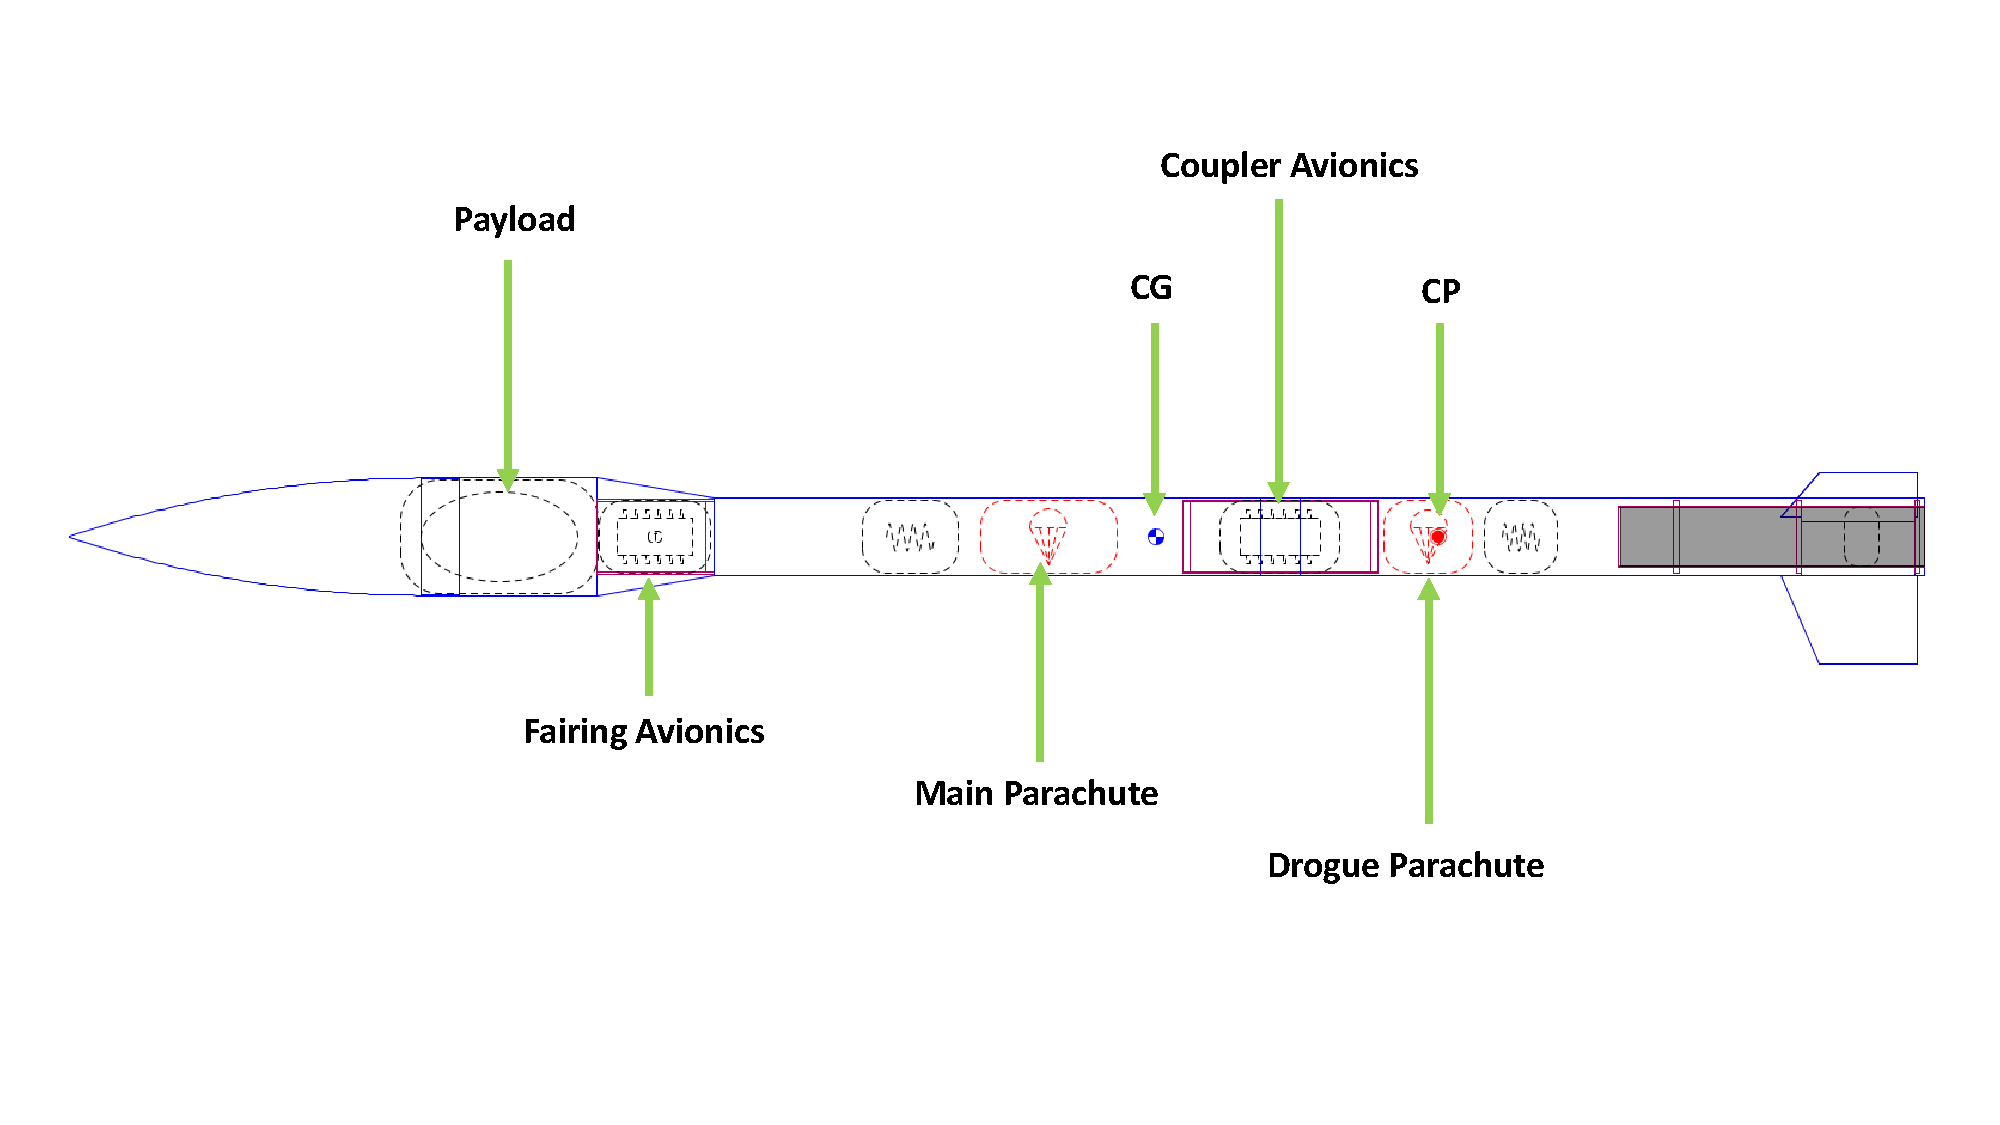
\includegraphics[width = 14cm, height = 7cm]{img/FIDO/openrocket_Model.pdf}
    \caption{OpenRocket model of launch vehicle, with various points of interest highlighted.}
    \label{fig:my_label}
\end{figure}   

\subsection{Kinetic Energy and Descent Time Predictions}
For each combination of launch parameters, the team simulated the trajectory of the launch vehicle under the spherical Earth condition (with time step 0.05s) and customized the simulations to yield data for the speed and altitude of the vehicle as functions of time. This data was used to demonstrate satisfactory flight duration and terminal kinetic energy. Specifically, the terminal specific kinetic energy was calculated using the following equation:
\begin{equation}
        t = \frac{v{_T}^2}{2}
\end{equation}
Where $v{_T}$ is the terminal velocity upon landing. Note that all components of the vehicle (lower body tube, upper body tube, and nose cone) are assumed to land at the same terminal velocity. The table below summarizes the data from these simulations that pertains to descent and landing.

\begin{table}[H]
    \centering
    \caption{Terminal descent characteristics for various launch parameters (spherical Earth condition)}
    \label{tab:FlightDynamics:TerminalDescentCharacteristics}
    \begin{tabularx}{\linewidth}{lllXX}
    \toprule
     \textbf{Angle [deg]} &  \textbf{Wind [mph]} &  \textbf{Descent time [s]} &  \textbf{Term. desc. velocity [m/s]} &  \textbf{Term. spec. kinetic energy [J/kg]} \\
    \midrule
       5.0 &     0 &        72.822 &               -7.4420 &                   27.691682 \\
       5.0 &     5 &        72.338 &               -7.4417 &                   27.689449 \\
       5.0 &    10 &        71.319 &               -7.4424 &                   27.694659 \\
       5.0 &    15 &        71.111 &               -7.4421 &                   27.692426 \\
       5.0 &    20 &        70.144 &               -7.4424 &                   27.694659 \\
       7.5 &     0 &        71.904 &               -7.4418 &                   27.690194 \\
       7.5 &     5 &        71.190 &               -7.4429 &                   27.698380 \\
       7.5 &    10 &        70.578 &               -7.4418 &                   27.690194 \\
       7.5 &    15 &        70.118 &               -7.4425 &                   27.695403 \\
       7.5 &    20 &        69.532 &               -7.4416 &                   27.688705 \\
      10.0 &     0 &        72.241 &               -7.4424 &                   27.694659 \\
      10.0 &     5 &        71.485 &               -7.4420 &                   27.691682 \\
      10.0 &    10 &        70.633 &               -7.4417 &                   27.689449 \\
      10.0 &    15 &        68.627 &               -7.4421 &                   27.692426 \\
      10.0 &    20 &        68.321 &               -7.4414 &                   27.687217 \\
    \bottomrule
    \end{tabularx}
\end{table}
The table shows that the descent time of the launch vehicle system in all simulated cases is well below the maximum allowed descent time of 90 seconds. Therefore, the team expects each of the components of the vehicle to descend from apogee within the maximum allowed time.
\\*
\newline
From the terminal specific kinetic energy data, the terminal kinetic energy can be calculated for each individual component by simply multiplying the specific kinetic energy by the mass of the component:
 \begin{equation}
    T{_c} = m{_c}*t    
 \end{equation}
To demonstrate that the impact kinetic energy requirement is satisfied, the team calculated the terminal kinetic energy of each component under the "worst-case scenario", or the simulated scenario with the highest terminal specific kinetic energy.  The results of these calculations are summarized in the table below.

\begin{table}[H]
\centering
\caption{Terminal kinetic energy of each component in worst-case scenario (spherical Earth condition)}
\label{tab:FlightDynamics:TerminalKineticEnergy}
\begin{tabularx}{.5\linewidth}{XlX}
\toprule
  \textbf{Component} & \textbf{Mass [kg]} &  \textbf{Term. kinetic energy [J]} \\
\midrule
Nose cone & 0.626 &             17.339186 \\
Fairing & 1.114 &             30.855996 \\
Upper body & 1.221 &             33.819722 \\
Switch band & 0.771 &             21.355451 \\
Lower body & 3.570 &             98.883217 \\
\bottomrule
\end{tabularx}
\end{table}

As can be seen, the terminal kinetic energy of each component (under the assumption that each component lands at the same terminal velocity) is less than the maximum allowed value of 101.69J (75ftlb). Therefore, according to OpenRocket, even under the most unfavorable launch characteristics, the launch vehicle still satisfies the impact energy requirement.

\subsection{Drift and Apogee Predictions}
The landing point of the launch vehicle is a critical safety concern to all parties and property in the area. To mitigate this risk, the team conducted several trajectory simulations for various wind speeds, launch angles, and simulation conditions. To visualize the drift, the trajectories were plotted on an in-plane graph, where the y-axis is north-south and the x-axis is east-west. The plots for the spherical Earth approximation condition are shown below.
\FloatBarrier
\begin{figure}[h]
    \centering
    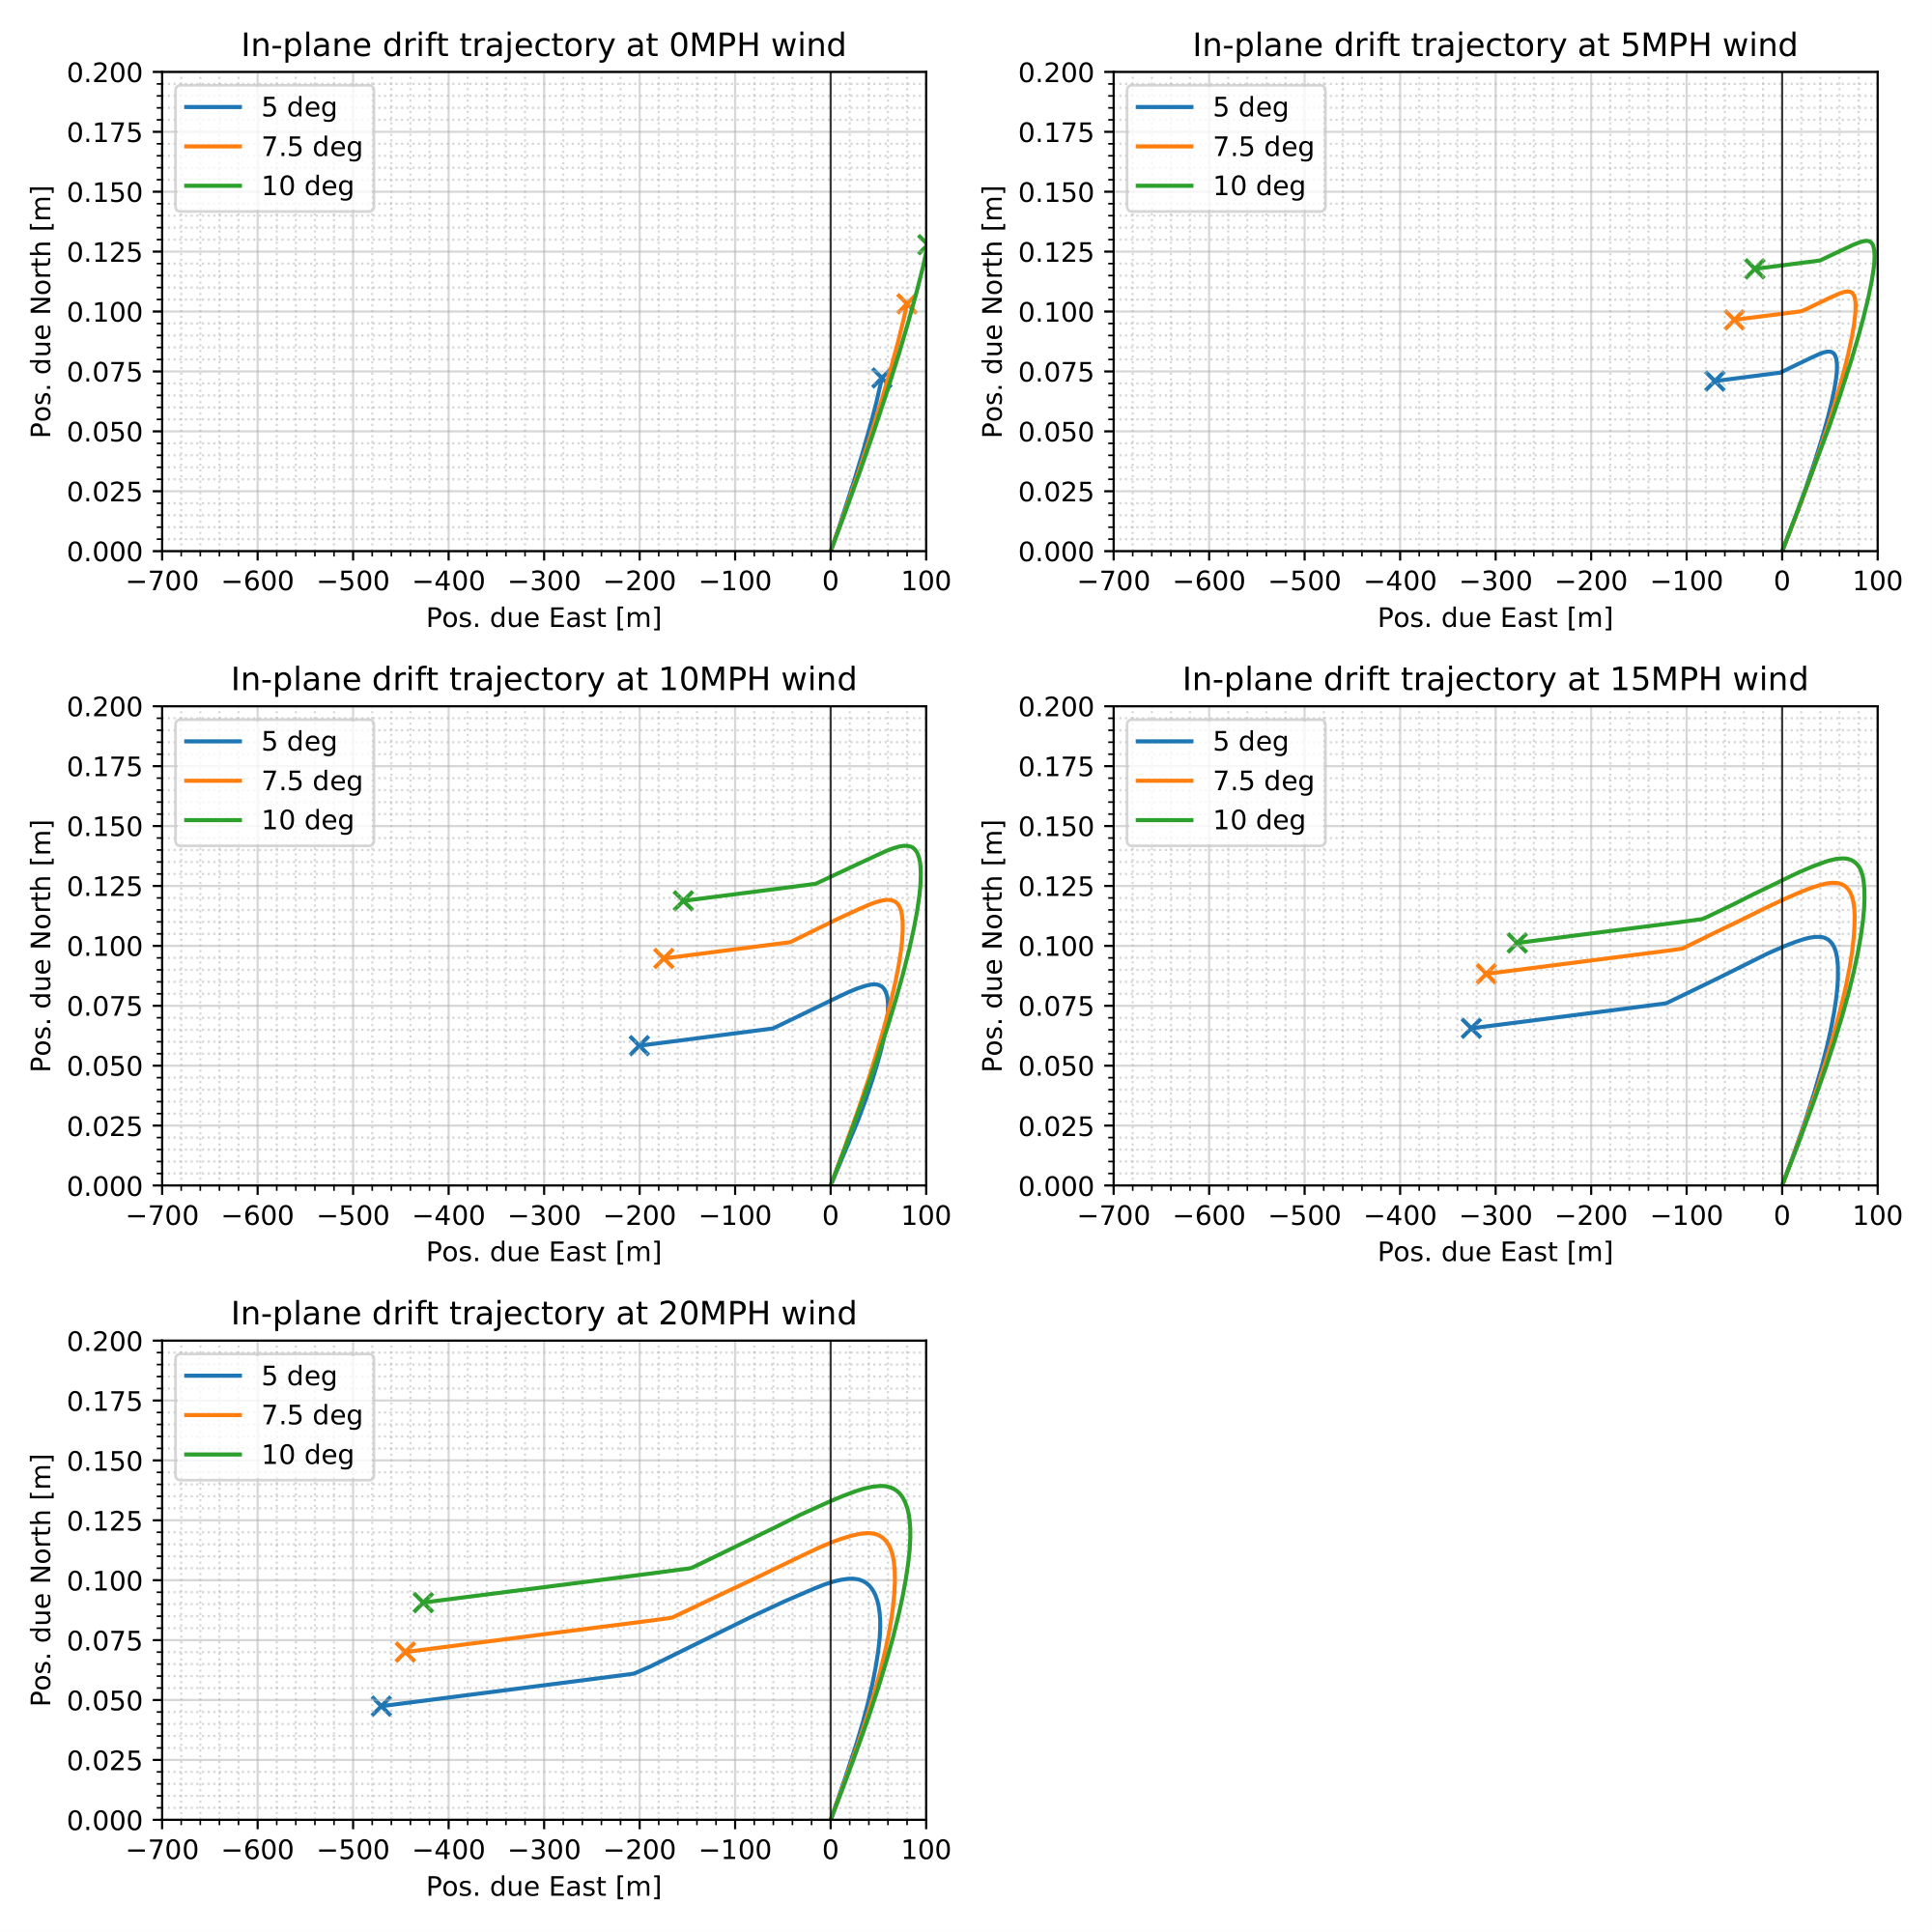
\includegraphics[width = 15cm, height = 11cm]{img/FIDO/InPlaneDrift-1.png}
    \caption{Predicted in-plane drift for various wind speeds and launch angles (all under spherical Earth approximation condition)}
    \label{fig:my_label}
\end{figure}
Note that, given the scaling of the north-south axis, the trajectories in each of these simulated scenarios is almost purely in the east-west direction. The most extreme landing displacement from the launch pad appears to occur in the 20-mph wind, 5 degree launch angle case, where the predicted landing distance from the launch pad is about 500m (about 1,640ft). Thus, even under the most extreme launch scenarios, the team expects the launch vehicle system to land well within the radius of the recovery area.
\\*
\newline
For the sake of comparison, the team conducted the exact same simulations for the WGS84 condition. The resulting plots are shown below.
\FloatBarrier
\begin{figure}[h]
    \centering
    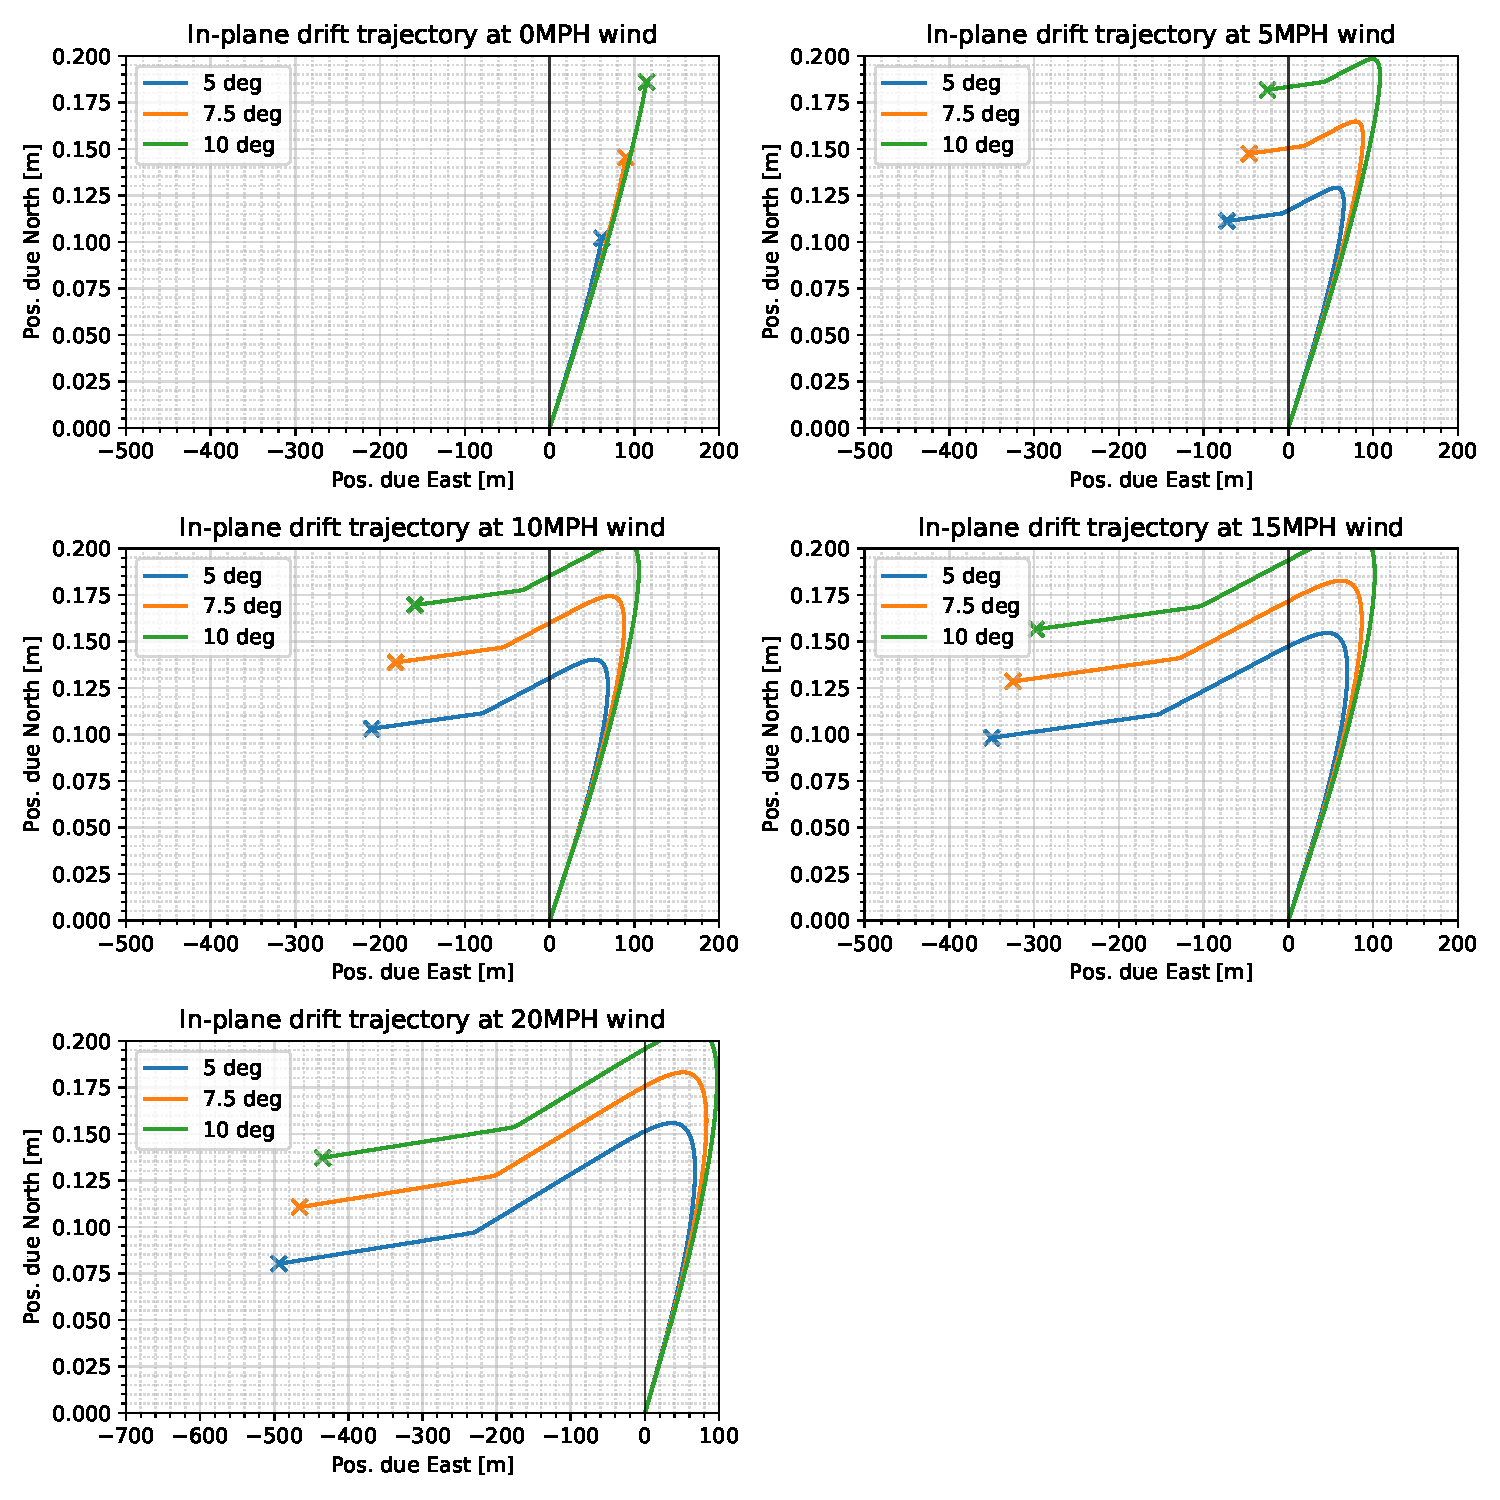
\includegraphics[width = 15cm, height = 11cm]{img/FIDO/InPlaneDriftWGS.pdf}
    \caption{Predicted in-plane drift for various wind speeds and launch angles (all under WGS84 condition)}
    \label{fig:my_label}
\end{figure}
\FloatBarrier
While the WGS84 and spherical Earth approximation conditions predict slightly different drift trajectories, neither of them predict a maximum possible landing distance from the launch pad over 500m (about 1,640ft), thus both simulation conditions provide compelling evidence that the launch vehicle system will land within the recovery area radius.
\\*
\newline
To determine the target apogee, the team also plotted the altitude data as a function of time from the same simulated trajectories.
\begin{figure}[h]
    \centering
    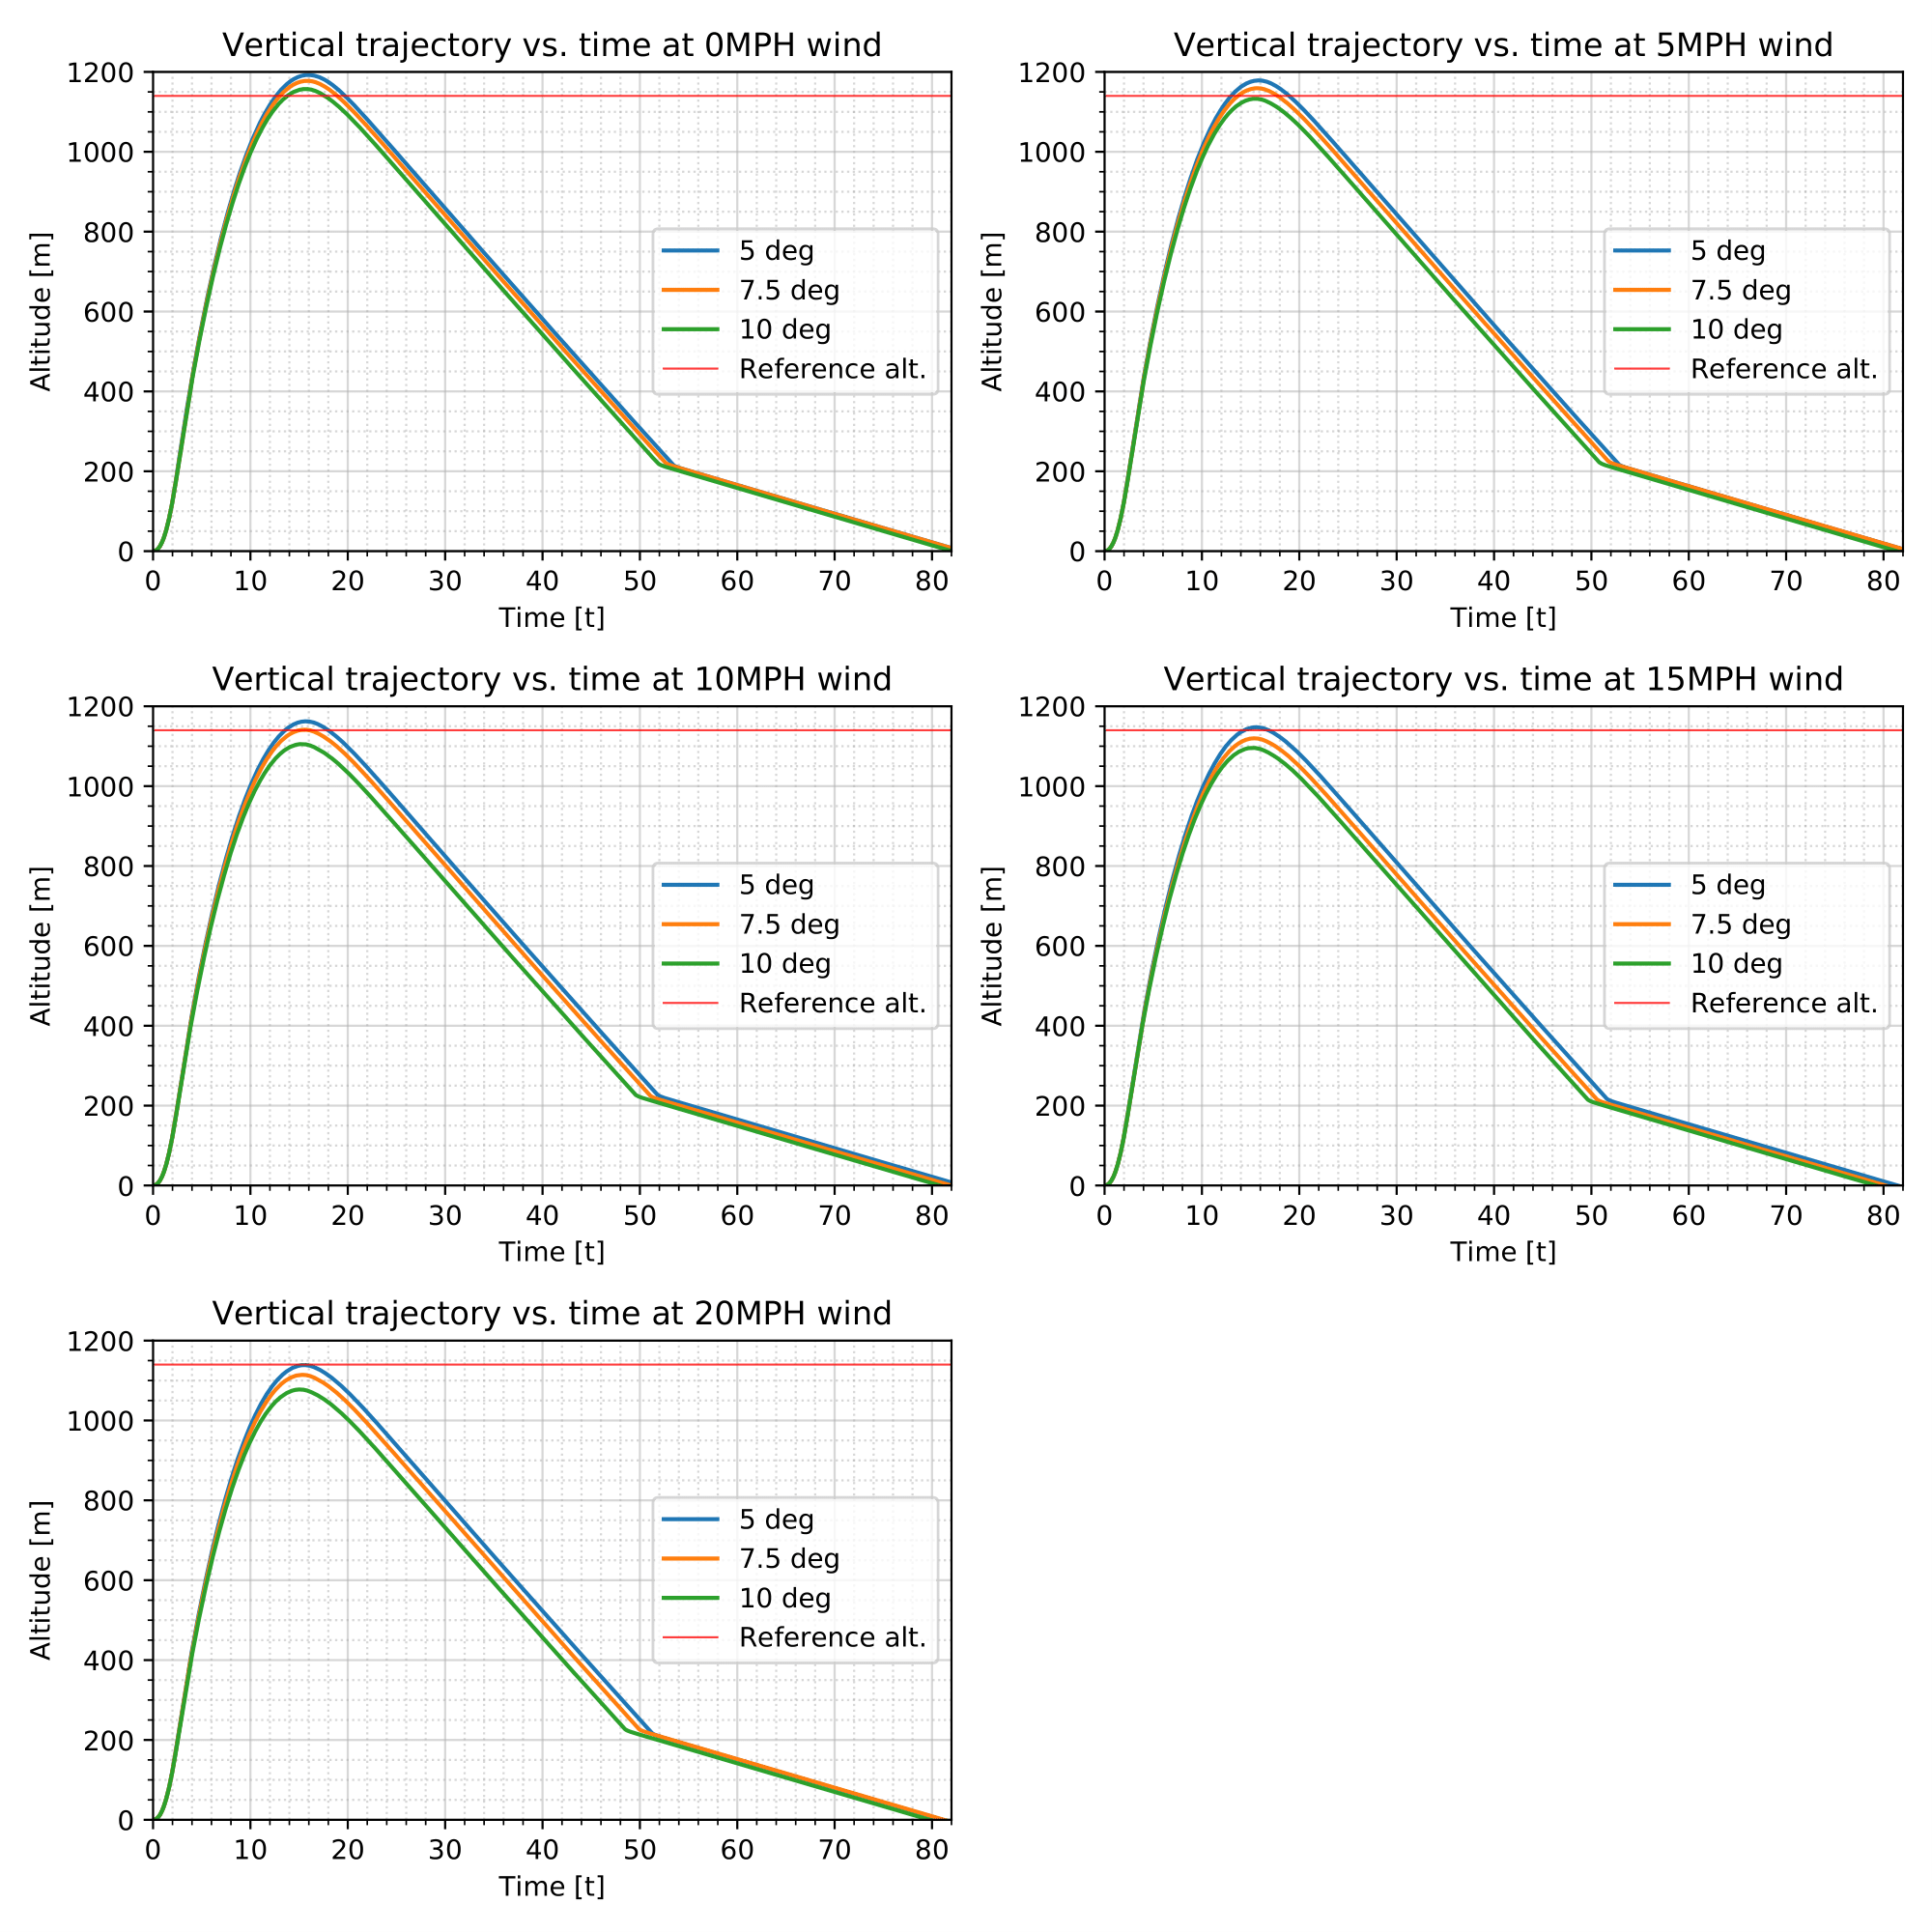
\includegraphics[width = 15cm, height = 11cm]{img/FIDO/VerticalTrajectory-1.png}
    \caption{Simulated altitude as a function of time for various wind conditions and launch angles (spherical Earth approximation condition)}
    \label{fig:my_label}
\end{figure}
\begin{figure}[h]
    \centering
    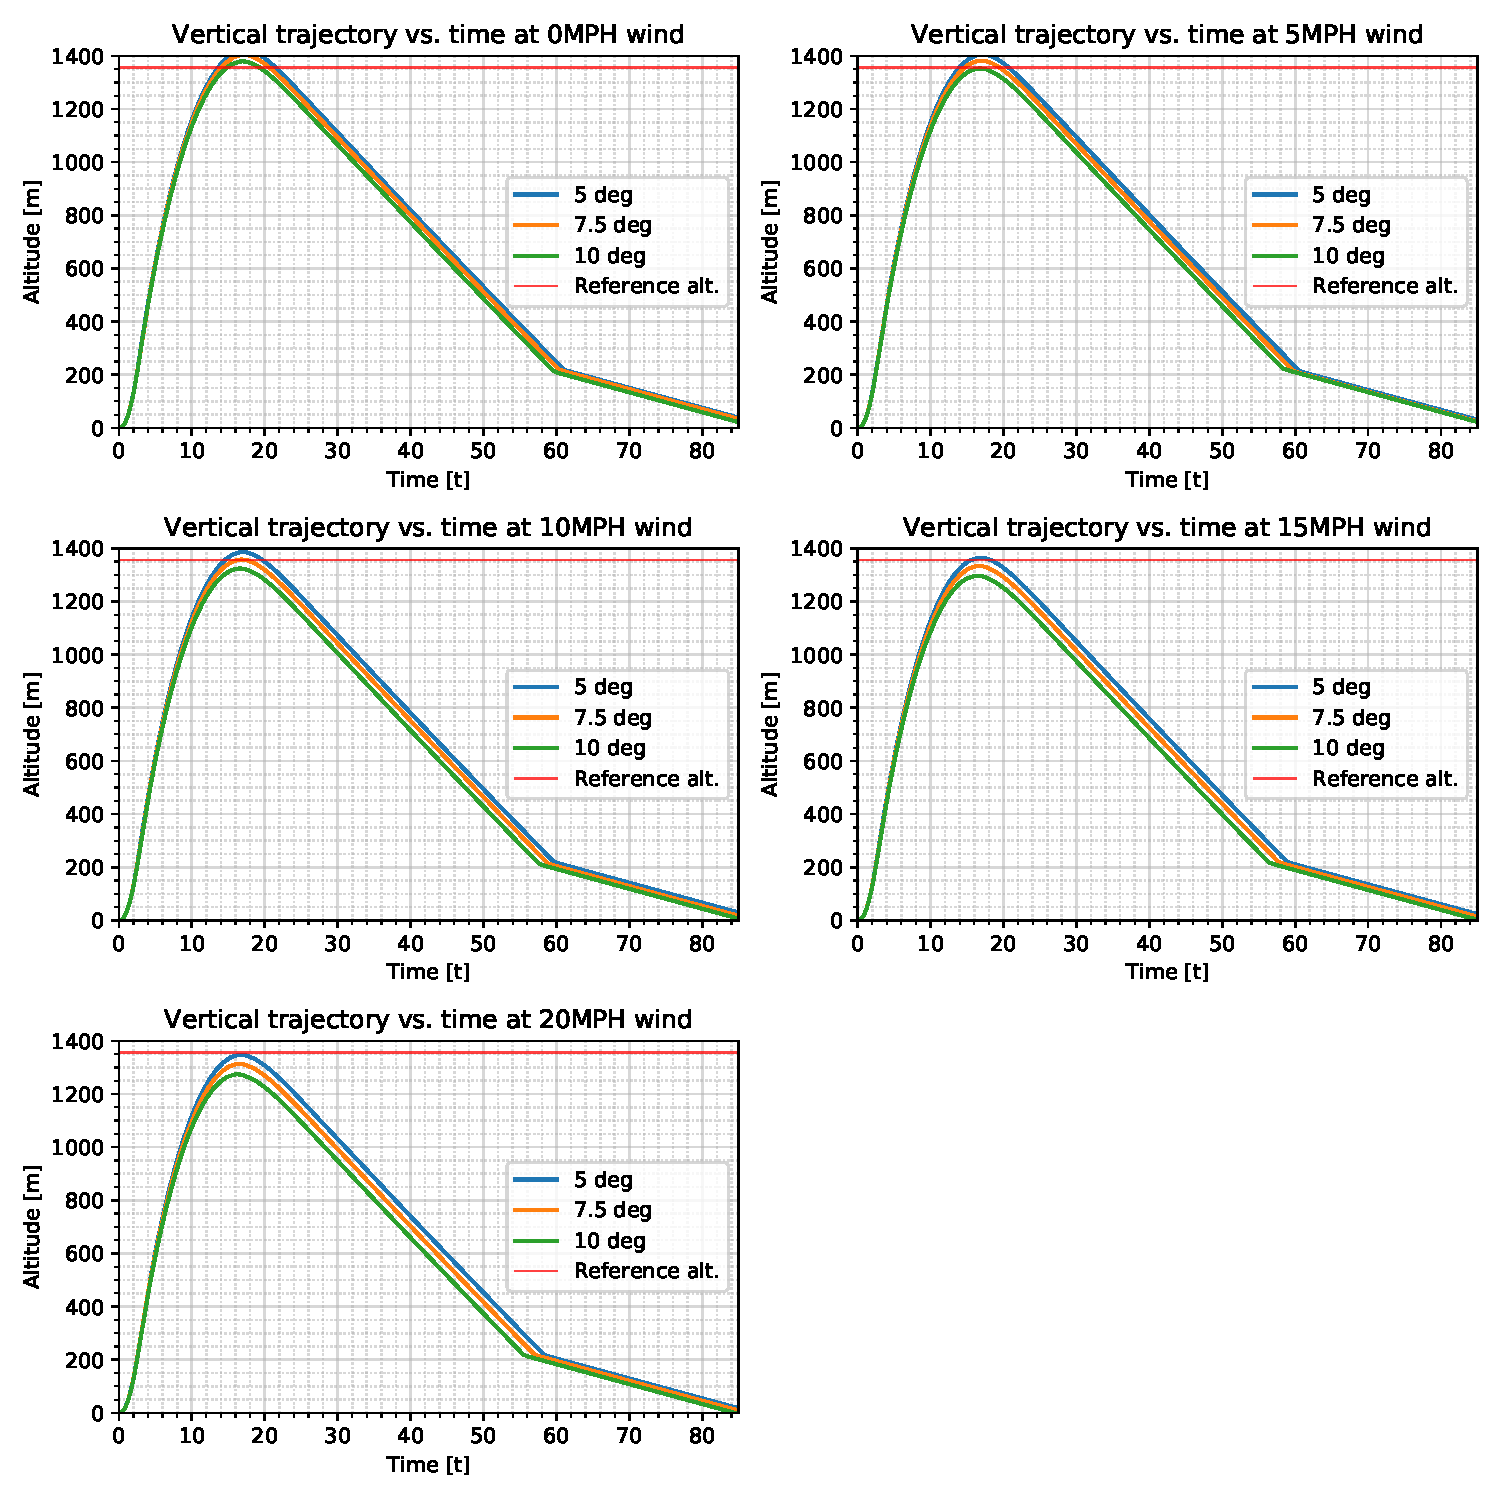
\includegraphics[width = 15cm, height = 11cm]{img/FIDO/VerticalTrajectoryWGS.pdf}
    \caption{Simulated altitude as a function of time for various wind conditions and launch angles (WGS84 condition)}
    \label{fig:my_label}
\end{figure}
\FloatBarrier
As can be seen in the plots above, the spherical Earth approximation and WGS84 conditions predictions of apogee differ significantly, in some cases by over 200m (over 656ft). However, as discussed previously, the WGS84 simulation condition is expected to be more accurate because it is a more accurate Earth model with a smaller time step size. As a result, the team primarily based its target altitude decision on the WGS84 simulation condition. The team has determined its official target altitude to be 4,450ft.
\begin{table}[H]
\centering
\caption{Official target altitude}
\label{tab:FlightDynamics:TargetAltitude}
\begin{tabularx}{.5\linewidth}{XlX}
\toprule
  \textbf{Target altitude [ft]}\\
\midrule
4,450 \\
\bottomrule
\end{tabularx}
\end{table}

\section{Simulation Discrepancies}
As the team ran simulations for the two different conditions (WGS84, spherical Earth approximation), the projected trajectories were typically found to have relatively minor discrepancies. To quantify the difference in results of the two simulation conditions, the time series data of altitude for each set of launch characteristics (launch angle and wind speed) from the spherical Earth approximation condition was subtracted from the WGS84 condition. This was done to calculate the root-mean-square (RMS) error of the difference between the two simulation conditions. The result of these calculations are shown in the table below.
\begin{table}[H]
\centering
\caption{Normalized root-mean-square error between the two simulation conditions for all launch parameters}
\label{tab:FlightDynamics:AverageError}
\begin{tabularx}{.5\linewidth}{llX}
\toprule
 \textbf{Angle [deg]} &  \textbf{Wind [mph]} &  \textbf{Error norm [m]} \\
\midrule
   5.0 &     0 &    0.558017 \\
   5.0 &     5 &    0.821123 \\
   5.0 &    10 &    0.906802 \\
   5.0 &    15 &    0.529063 \\
   5.0 &    20 &    0.567203 \\
   7.5 &     0 &    1.070750 \\
   7.5 &     5 &    0.152635 \\
   7.5 &    10 &    0.350443 \\
   7.5 &    15 &    0.332065 \\
   7.5 &    20 &    0.547357 \\
  10.0 &     0 &    1.646402 \\
  10.0 &     5 &    0.161091 \\
  10.0 &    10 &    1.463531 \\
  10.0 &    15 &    0.613284 \\
\bottomrule
\end{tabularx}
\end{table}
As can be seen, the average difference in predicted altitude over time between the two simulation conditions across all sets of simulated launch parameters (launch angle and wind speed) never exceeded 2m. Thus, the team is confident that the simulated trajectories provided by OpenRocket are sufficiently reliable to guide further design considerations and developments of the launch vehicle and mission profile. 